\documentclass[border=10pt]{standalone}
\newcommand{\stB}{B}
\usepackage{tikz}
\tikzset{
  treenode/.style = {shape=rectangle, rounded corners,
                     draw, align=center,
                     top color=green!50, bottom color=green!50},
  root/.style     = {treenode, font=\Large, top color=red!50, bottom color=red!40},
  env/.style      = {treenode},
  env1/.style     = {treenode, top color=blue!50, bottom color=blue!50},
  dummy/.style    = {circle,draw}
  
}
\begin{document}
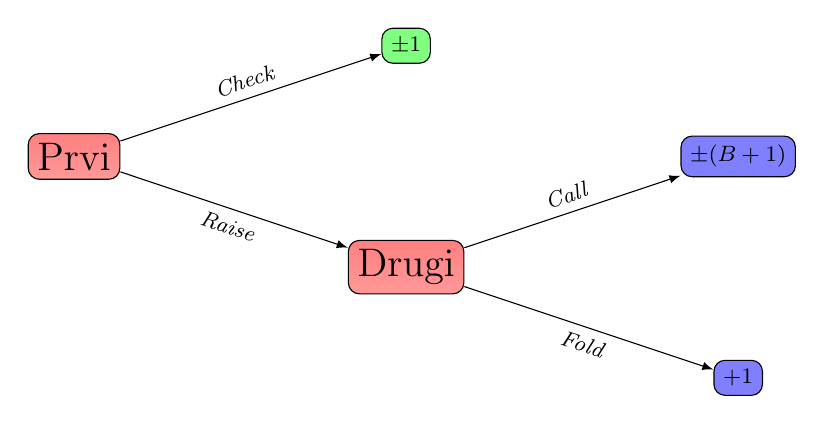
\begin{tikzpicture}
  [
    grow                    = right,
    sibling distance        = 8em,
    level distance          = 12em,
    edge from parent/.style = {draw, -latex},
    every node/.style       = {font=\footnotesize},
    sloped
  ]
  \node [root] {Prvi}
    child {node [root] {Drugi}
        child{node [env1] {$+1$}
        edge from parent node [below] {\emph{Fold}}} 
        child{node [env1]{$\pm(\stB+1)$}
        edge from parent node [above] {\emph{Call}}}
        edge from parent node [below] {\emph{Raise}}}
    child {node [env] {$\pm1$}
        edge from parent node [above] {\emph{Check}} };
\end{tikzpicture}
kokoko
\end{document}